We choose to work with 3 datasets and combination of 2 of them (section 2.1) \newline
In preprocessing data, we decide to use image processing to enhance image and extract features in order to speed up our model. \newline
Used methods: \newline
\begin{itemize}
\item \textbf{HOG \textit{“histogram of gradients”} } We use \textbf{skimage} library to handle this because it allow more control over HOG parameters, our HOG parameters are: 8 bins for the histogram, 12X12 pixels per cell, 4X4 cells per block with disabled multichannel as we train the model on gray scale images.
we tried different normalization methods on the different datasets we had and chose the one that gave a better result on average.

\begin{center}
	\begin{tabular}{ c|c|c|c }
		& FER & CK+ & RafD \\ \hline
		L1-norm & 23.16\% & 36.11\% & 89.08\% \\  
		L2-norm & 36.80\% & 57.33\% & \textbf{90.2\%} \\
		L1-sqrt & \textbf{38.61\%} & 46.83\% & 89.21\% \\
		L2-Hys & \textbf{38.61\%} & \textbf{57.99\%} & 88.96\% \\
	\end{tabular}
\end{center}
With FER \textbf{L1-sqrt} and \textbf{L2-Hys} give best result.\newline
With CK+ we choose to work with  .\newline
With RafD we choose to work with  \textbf{L2-norm}. (we chose this as it gave best results on \textbf{RafD} dataset and very acceptable results on average)\newline
as obvious from the results \textbf{L1-sqrt} and \textbf{L2-Hys} methods tend to show better results on average, but \textbf{L2-Hys} seems to be more effective method.\newline

\item \textbf{Face landmarks } We use \textbf{DLIB} library with trained model to extract \textbf{68 face landmarks} from each face we pass to it, There are 2 models also, one with 5 landmarks and this isn’t enough for our model and one with 194 landmarks “this could be perfect, but it is size is too large”\footnote{
	we use hog and face landmarks according to instructions paper\cite{method_5}, we get this from \cite{state_of_art} (paper compares papers in facial emotion recognition), this paper claims that its accuracy 70\% but after many trials we only reached a maximum accuracy of 57.63\% with FER dataset.
}.

	\item \textbf{Face detection} We worked with pre-trained models like \textit{HAAR}, \textit{LBP} cascading classifiers and \textit{DLIB detector}, they work with frontal face and each one has its own advantages, HAAR is quite accurate but slow, LBP is faster than HAAR but less accurate and DLIB detector is more accurate than HAAR and detection time depends on the image size so our default classifier is DLIB detector. 
	
	\item \textbf{Image enhancement} In the training phase we have to ensure that all the input image is gray scale and all of them is the same size, For noise removal, we only work with gaussian noise(by fastNLMeans algorithm) and salt \& pepper noise(with median filter).
\end{itemize}

\paragraph{Model Results}
\begin{enumerate}
\item For \textit{FER} dataset \newline
\begin{itemize}[noitemsep,nolistsep]
    \item Only CNN: Its training accuracy is 90.07\% and testing accuracy is 75.38\%.

	\begin{comment}
    \item Only HOG: 
        \begin{itemize}
            \item It takes X time in training and X time in testing.
            \item The model size was 966 KB.
            \item Its training accuracy is 72.33\% and testing accuracy is 53.9\%.
        \end{itemize}
    \item Only landmarks: 
        \begin{itemize}
            \item It takes X time in training and X time in testing.
            \item The model size was X.
            \item Its training accuracy is X and testing accuracy is X.
        \end{itemize}
	\end{comment}

    \item HOG and landmarks: Its training accuracy is 86.1\% and testing accuracy is 55\%.
    \item CNN, HOG and landmarks: Its training accuracy is 94.17\% and testing accuracy is 58.08\%.
\end{itemize}

\item For \textit{CK+} dataset \newline
\begin{itemize}[noitemsep,nolistsep]
    \item Only CNN: using 5 Expochs, Its training accuracy is 100\% and testing accuracy is 85.13\%.

	\begin{comment}
    \item Only HOG: 
        \begin{itemize}
            \item It takes X time in training and X time in testing.
            \item The model size was X.
            \item Its training accuracy is X and testing accuracy is X.
        \end{itemize}
    \item Only landmarks: 
        \begin{itemize}
            \item It takes X time in training and X time in testing.
            \item The model size was X.
            \item Its training accuracy is X and testing accuracy is X.
        \end{itemize}
	\end{comment}

    \item HOG and landmarks: Its training accuracy is 100\% and testing accuracy is 88.4\%.
    \item CNN, HOG and landmarks: Its training accuracy is 92\% and testing accuracy is 85\%.
\end{itemize}
\item For \textit{RafD} dataset \newline
\begin{itemize}[noitemsep,nolistsep]
    \item Only CNN: Its training accuracy is 95\% and testing accuracy is 89.04\%.

	\begin{comment}
    \item Only HOG: 
        \begin{itemize}
            \item It takes X time in training and X time in testing.
            \item The model size was X.
            \item Its training accuracy is X and testing accuracy is X .
        \end{itemize}
    \item Only landmarks: 
        \begin{itemize}
            \item It takes X time in training and X time in testing.
            \item The model size was X.
            \item Its training accuracy is X and testing accuracy is X.
        \end{itemize}
	\end{comment}

    \item HOG and landmarks: Its training accuracy is 100\% and testing accuracy is 92.83\% .
    \item CNN, HOG and landmarks: Its training accuracy is 100\% and testing accuracy is 93\%.
\end{itemize}

\item For \textit{CK+ and RafD} combination \newline
\begin{itemize}[noitemsep,nolistsep]
    \item Only CNN: Its training accuracy is 98.2\% and testing accuracy is 87.8\%.

	\begin{comment}
    \item Only HOG: 
        \begin{itemize}
            \item It takes X time in training and X time in testing.
            \item The model size was X.
            \item Its training accuracy is X and testing accuracy is X.
        \end{itemize}
    \item Only landmarks: 
        \begin{itemize}
            \item It takes X time in training and X time in testing.
            \item The model size was X.
            \item Its training accuracy is X and testing accuracy is X.
        \end{itemize}
	\end{comment}

    \item HOG and landmarks: training accuracy is 99.89\% and testing accuracy is 98.43\%.
    \item CNN, HOG and landmarks: training accuracy is 100\% and testing accuracy is 89.74\%.
\end{itemize}
\end{enumerate}
%\newpage
\paragraph{Confusion matrices}
this section will include the confusion matrices on all data sets we tried using the model trained on HOG and landmarks only.
\begin{itemize}
	\item for FER data set:
		\begin{itemize}
			\item on 7 basic emotions\footnote{Happiness, Sadness, Anger, Disgust, Fear, Surprise, Neutral}.
			\begin{figure}[H]
				\centering
				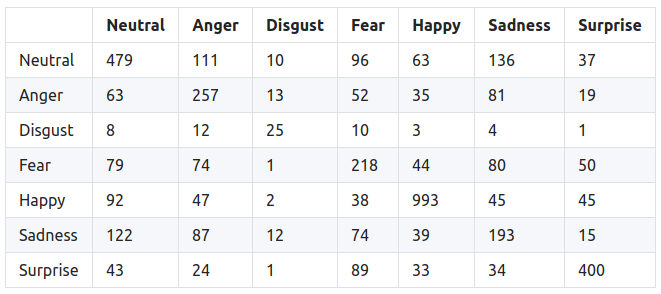
\includegraphics[width=0.75\textwidth]{images/fer_long.png}
			\end{figure}
		
			\item on 3 emotions only\footnote{Satisfied, Unsatisfied, neural}.
			\begin{figure}[H]
				\centering
				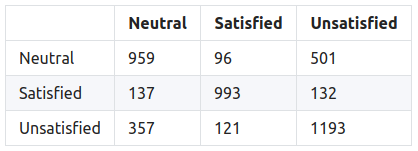
\includegraphics[width=0.75\textwidth]{images/fer_short.png}
			\end{figure}
		\end{itemize}
		
	\item for CK+ data set:
		\begin{itemize}
			\item on 8 basic emotions\footnote{Happiness, Sadness, Anger, Disgust, Fear, Surprise, Neutral, Contempt}.
			\begin{figure}[H]
				\centering
				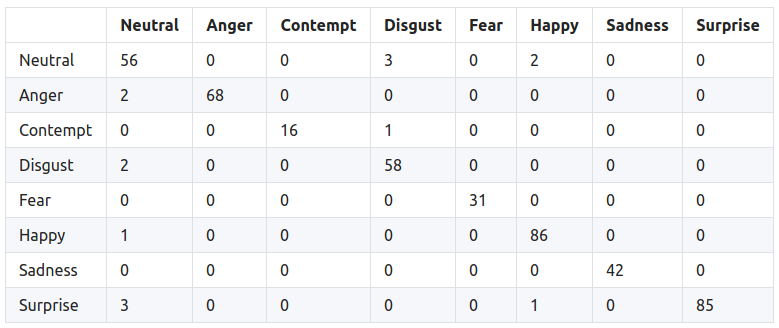
\includegraphics[width=0.75\textwidth]{images/ck_long.png}
			\end{figure}
			
			\item on 3 emotions only.
			\begin{figure}[H]
				\centering
				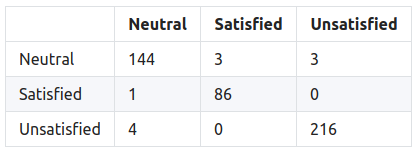
\includegraphics[width=0.75\textwidth]{images/ck_short.png}
			\end{figure}
		\end{itemize}
	\item for RafD data set:
		\begin{itemize}
			\item on 8 basic emotions.
			\begin{figure}[H]
				\centering
				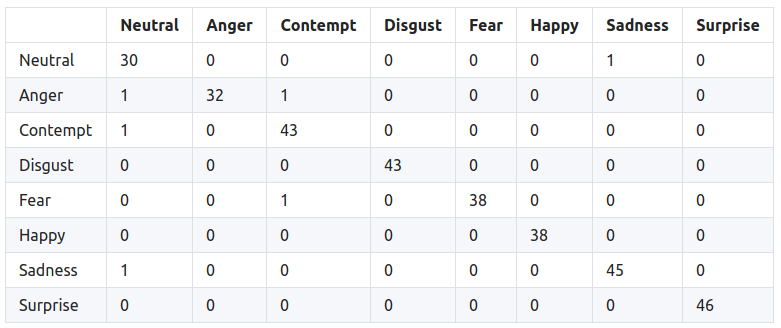
\includegraphics[width=0.75\textwidth]{images/rafd_long.png}
			\end{figure}
			
			\item on 3 emotions only.
			\begin{figure}[H]
				\centering
				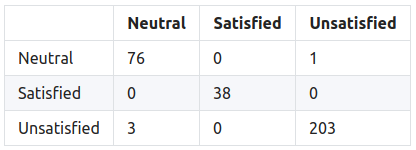
\includegraphics[width=0.75\textwidth]{images/rafd_short.png}
			\end{figure}
		\end{itemize}
	\item for Combined data set:
		\begin{itemize}
			\item on 8 basic emotions.
			\begin{figure}[H]
				\centering
				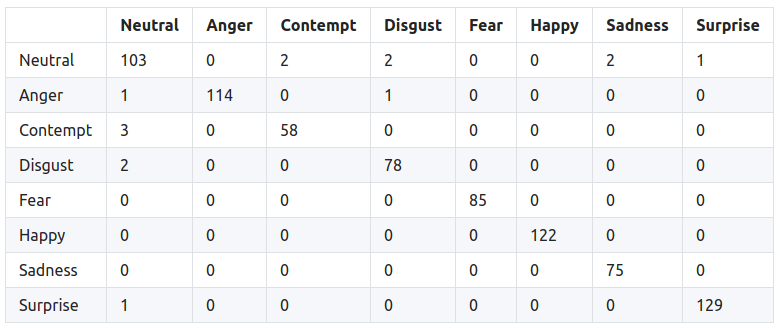
\includegraphics[width=0.75\textwidth]{images/combined_long.png}
			\end{figure}
			%\newpage
			\item on 3 emotions only.
			\begin{figure}[H]
				\centering
				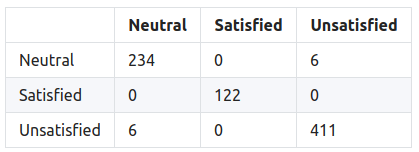
\includegraphics[width=0.75\textwidth]{images/combined_short.png}
			\end{figure}
		\end{itemize}
\end{itemize}
